\section{数据预处理与特征分析}
\label{sec:data-analysis}

本节对原始数据进行清洗与特征提取。首先统一数据的时间基准，确保各维变量在同一物理时间轴上严格对齐；随后深入挖掘数据的周期性、低秩性及预报误差分布特征，为后续预测模型的设计与融合策略提供直接的数据支撑。

\subsection{数据质量检查与时间基准统一}

附件2（负荷与实际光伏）与附件4（动态电价）均为2025全年数据，按10分钟间隔划分为144个区间，全年共52560个观测值。为统一口径，时间戳定义为区间结束时刻（如00:10对应00:00--00:10，``0:00+1''对应次日00:00），由此构建2025年1月1日00:10至2026年1月1日00:00的连续时间轴，以保证功率平衡、储能状态递推与购电结算基准一致。

数据核验显示各附件完整、无缺失值、异常负值及时间戳冲突；附件3日期列空白为同日批次正常沿用。针对附件3的小时级光伏预报，本文采用保持局部单调性的PCHIP插值降尺度至10分钟网格，且严格以发布时刻已知实测值为起点，避免未来信息泄露。功率统一以kW计，区间电量按$\mathrm{kWh}=\mathrm{kW}\times\Delta t$（$\Delta t=1/6\,\mathrm{h}$）换算，电价统一为元/kWh。

\subsection{负荷与光伏的周期性分析}

分别计算10分钟序列在滞后1天（144步）和7天（1008步）的Pearson相关系数。负荷的日、周相关系数分别为0.6792和0.9855，表现出强烈的周重复性；光伏全序列的日、周相关系数分别高达0.9923和0.9903。剔除夜间无光照时段后，光伏的日、周相关系数仍达0.9845和0.9789，周期特征依然显著（见图\ref{fig:data-periodicity}）。该特征表明，后续建模应充分利用日轮廓与一周时滞相关结构（如引入“上周同刻”特征）作为预测依据。

\begin{figure}[H]
  \centering
  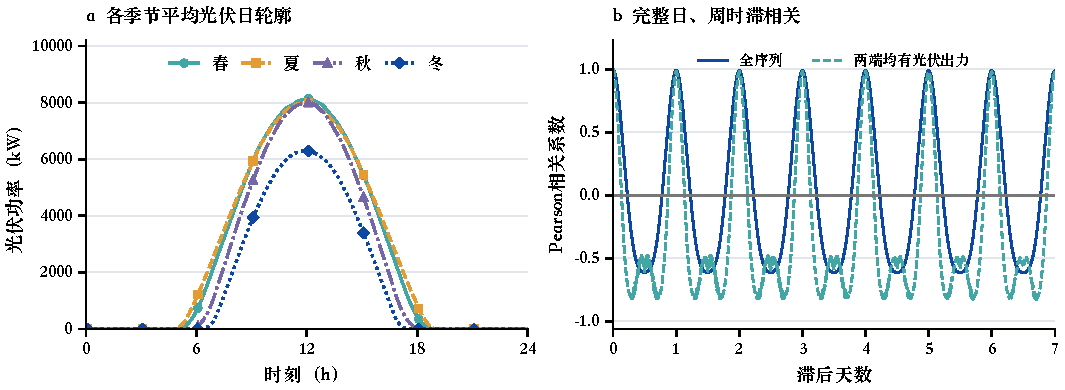
\includegraphics[width=0.94\textwidth]{figures/redesign/fig_periodicity.pdf}
  \caption{光伏季节性日轮廓与一周时滞相关结构}
  \label{fig:data-periodicity}
\end{figure}

\subsection{光伏序列的低秩性分析}

构建连续7天光伏历史窗口的Hankel矩阵并进行奇异值分解\cite{qiu2013matrix}。如图\ref{fig:hankel-spectrum}所示，奇异值呈现快速衰减趋势，前几个奇异值集中了绝大部分的谱能量。奇异值的快速衰减表明，光伏历史序列的主要变化可以由少量谱成分表示，具有较明显的低秩近似特征。因此，后续将低秩矩阵方法纳入候选预测模型。

\begin{figure}[H]
  \centering
  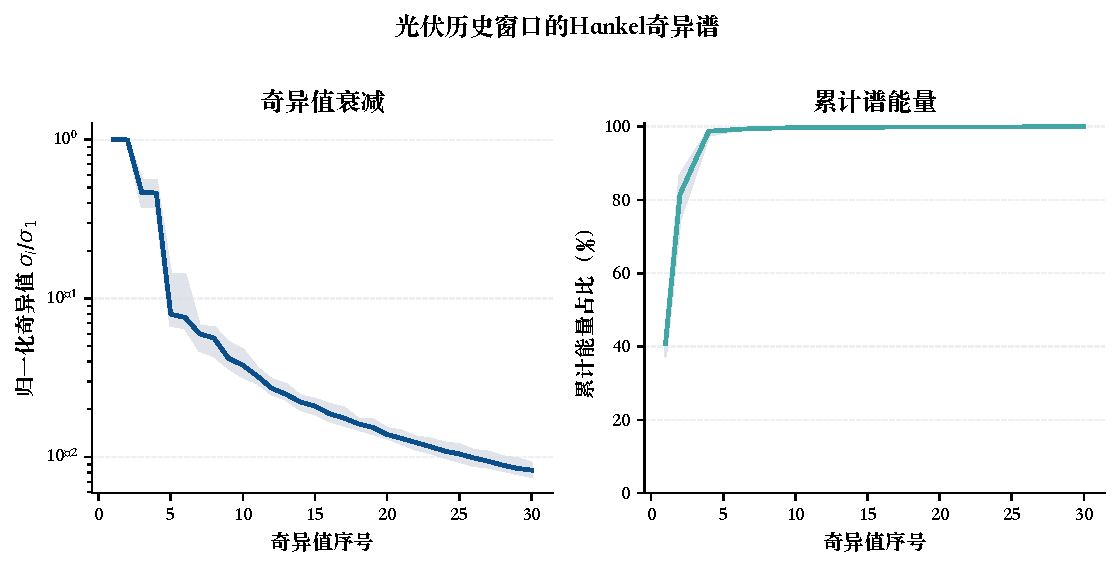
\includegraphics[width=0.88\textwidth]{figures/common/fig_hankel_spectrum.pdf}
    \caption{52个连续7天光伏历史窗口的Hankel奇异谱}
  \label{fig:hankel-spectrum}
\end{figure}

\subsection{官方光伏预报误差的提前期效应}

将附件3中35004个与实际光伏对齐的预报目标按提前期（1--3 h、4--6 h、7--12 h、13--18 h、19--24 h）进行分组统计。结果显示（图\ref{fig:official-lead-error}），各组的MAE依次为34.53、77.78、144.79、226.29和319.51 kW，RMSE依次为69.43、170.45、298.88、458.91和673.02 kW。官方预报误差随提前期延长呈显著放大趋势。这表明不同提前期的预报置信度存在本质差异，后续的模型融合不应采用固定权重，而须引入基于提前期的分段策略。

\begin{figure}[H]
  \centering
  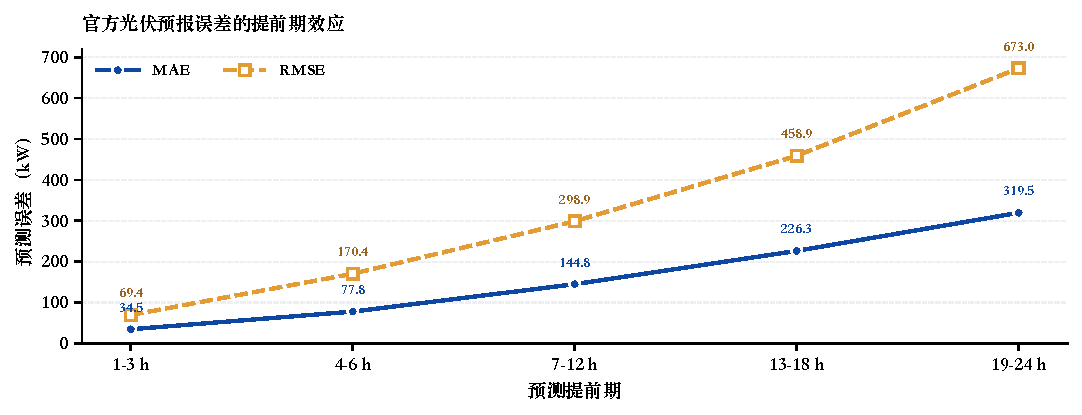
\includegraphics[width=0.86\textwidth]{figures/redesign/fig_data_official_lead_error.pdf}
    \caption{官方光伏预报误差的提前期效应}
  \label{fig:official-lead-error}
\end{figure}

\subsection{数据分析对模型构建的启示}

基于上述结构诊断与数据挖掘，本文提炼出三条核心建模准则：
\begin{enumerate}
  \item \textbf{强周期性驱动：}负荷与光伏的日、周相关性较高，支持将季节模型纳入基准候选集；
  \item \textbf{低秩结构利用：}Hankel奇异谱快速衰减，支持用低秩矩阵结构降噪与趋势预测；
  \item \textbf{动态置信度融合：}官方预报误差随提前期递增的规律，确立了采用“按提前期分段融合”策略的必要性。
\end{enumerate}
